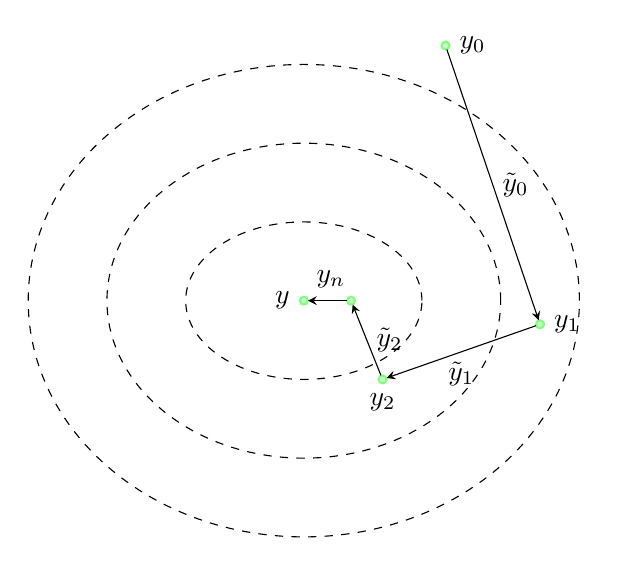
\begin{tikzpicture}
    [place/.style={circle,scale=0.3,draw=green!50,fill=green!20,thick},
    transition/.style={rectangle,draw=black!50,fill=black!20,thick}]

    %\draw[help lines] (-2.9,-0.2) grid (2.9,3.9);
    \draw[dashed] (0,0) circle [x radius=1.5, y radius=1];
    \draw[dashed] (0,0) circle [x radius=2.5, y radius=2];
    \draw[dashed] (0,0) circle [x radius=3.5, y radius=3];
    %\draw[dashed,thin] (0,0) circle [x radius=4.5, y radius=4];

    \node[place,label=right:{$y_0$}] (f0) at (1.8,3.24)  {};
    \node[place,label=right:{$y_1$}] (f1) at (3.0,-0.3)  {};
    \node[place,label=below:{$y_2$}] (f2) at (1.0,-1.0)   {};
    \node[place] (f3) at (0.6,0.0)   {};
    \node[place,label=left:{$y$},label=north east:{$y_n$}] (fn) at (0,0)  {};

    \draw[->,>=stealth] (f0) -- (f1) node[midway,right] {$\tilde{y}_0$};
    \draw[->,>=stealth] (f1) -- (f2) node[midway,below] {$\tilde{y}_1$};
    \draw[->,>=stealth] (f2) -- (f3) node[midway,right] {$\tilde{y}_2$};
    \draw[->,>=stealth] (f3) -- (fn);
\end{tikzpicture}
